\documentclass[12pt]{article}
\usepackage[margin=2.5cm]{geometry}
\usepackage{enumerate}
\usepackage{amsfonts}
\usepackage{amsmath}
\usepackage{fancyhdr}
\usepackage{amsmath}
\usepackage{amssymb}
\usepackage{amsthm}
\usepackage{mdframed}
\usepackage{graphicx}
\usepackage{subcaption}
\usepackage{adjustbox}
\usepackage{listings}
\usepackage{xcolor}
\usepackage{booktabs}
\usepackage[utf]{kotex}
\usepackage{hyperref}

\definecolor{codegreen}{rgb}{0,0.6,0}
\definecolor{codegray}{rgb}{0.5,0.5,0.5}
\definecolor{codepurple}{rgb}{0.58,0,0.82}
\definecolor{backcolour}{rgb}{0.95,0.95,0.92}

\lstdefinestyle{mystyle}{
    backgroundcolor=\color{backcolour},
    commentstyle=\color{codegreen},
    keywordstyle=\color{magenta},
    numberstyle=\tiny\color{codegray},
    stringstyle=\color{codepurple},
    basicstyle=\ttfamily\footnotesize,
    breakatwhitespace=false,
    breaklines=true,
    captionpos=b,
    keepspaces=true,
    numbers=left,
    numbersep=5pt,
    showspaces=false,
    showstringspaces=false,
    showtabs=false,
    tabsize=1
}

\lstset{style=mystyle}

\pagestyle{fancy}
\renewcommand{\headrulewidth}{0.4pt}
\lhead{Hyungmo Gu}
\rhead{CSC369 Week 10 Notes}

\begin{document}
\title{CSC369 Week 10 Notes}
\author{Hyungmo Gu}
\maketitle

\begin{itemize}
    % \item Remember Example from Last Week?
    % \item Types of Resources
    % \item Not Just an OS Problem
    \item Deadlock Defined
    \begin{itemize}
        \item \textbf{Google Definition:} Is a situation one typically involving
        opposing parties, in which no progress can be made.
        \item Is permanent
        \item Happens to set of processes that

        \begin{itemize}
            \item Compete for same system resources
            \item Communicate with each other
        \end{itemize}
    \end{itemize}
    \item Example of Deadlock
    \begin{itemize}
        \item Law passed by Kansas Legislature in in early 20th century
        \begin{itemize}
            \item ``When two trains approach each other at a crossing, both shall
            come to a full stop and \underline{neither} shall start upon again
            until the other is gone''
        \end{itemize}
    \end{itemize}

    \begin{center}
        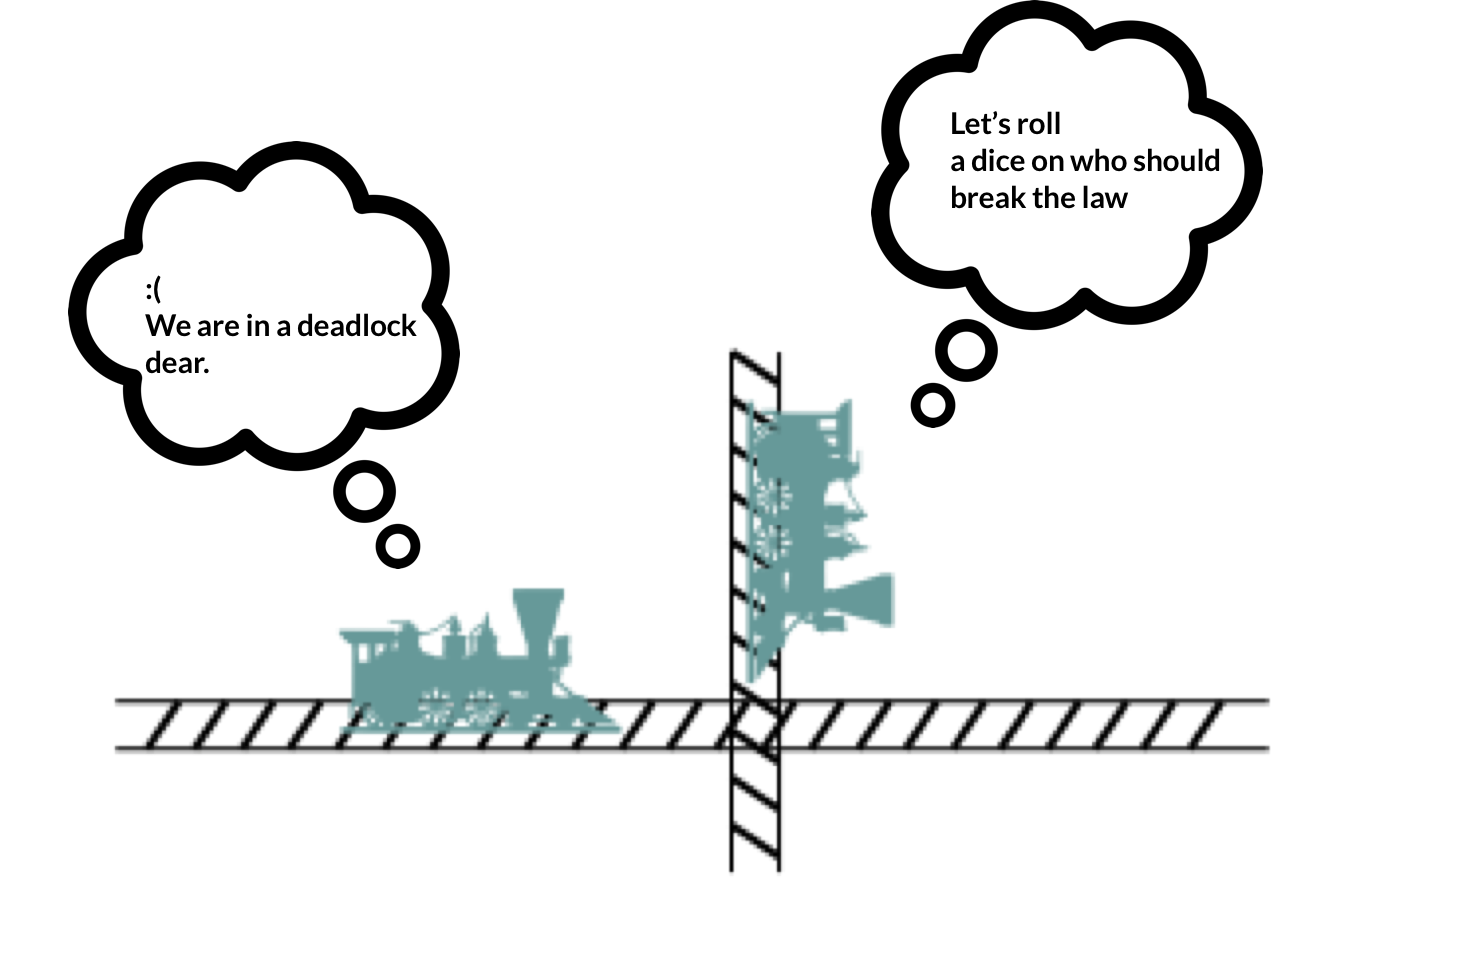
\includegraphics[width=0.8\linewidth]{images/week_10_notes_1_1.png}
    \end{center}


    % \item Example: Dining Philosopers
    % \item Deadlock Continued
    \item Conditions for Deadlock
    \begin{itemize}
        \item Neccesary and Sufficient Conditions
        \begin{enumerate}[1.]
            \item Mutual Exclusion
            \begin{itemize}
                \item Only one process may use a resource at a time
            \end{itemize}
            \item Hold and wait
            \begin{itemize}
                \item A process may hold allocated resources while awaitng
                assignment of others
            \end{itemize}
            \item No preemption
            \begin{itemize}
                \item No Resource can be forcibly removed from a process holding
                it
            \end{itemize}
            \item Circular wait
            \begin{itemize}
                \item Each process must be waiting for a resource which is being
                held by another process, which in turn is waiting for the first
                process to release the resource $^{[3]}$
            \end{itemize}
        \end{enumerate}
    \end{itemize}

    \bigskip

    \begin{mdframed}
        \underline{\textbf{Aside}}

        \bigskip

        \begin{enumerate}
            \item Wait. Necessary condition? $^{[1]}$
            \begin{itemize}
                \item We say $N$ is a necessary condition for $S$ if we don't have $N$,
                we won't have $S$.
            \end{itemize}
            \item Wait. Sufficient condition? $^{[1]}$
            \begin{itemize}
                \item We say $S$ is a necessary condition for $N$ if we have $S$,
                then we know that $N$ must follow, i.e. $S \Rightarrow N$
            \end{itemize}
            \item Hold on. How about necessary and sufficient condition? $^{[2]}$
            \begin{itemize}
                \item Is when necessary and sufficient conditions are put together
                similar to if and only if $^{[2]}$

                \begin{center}
                    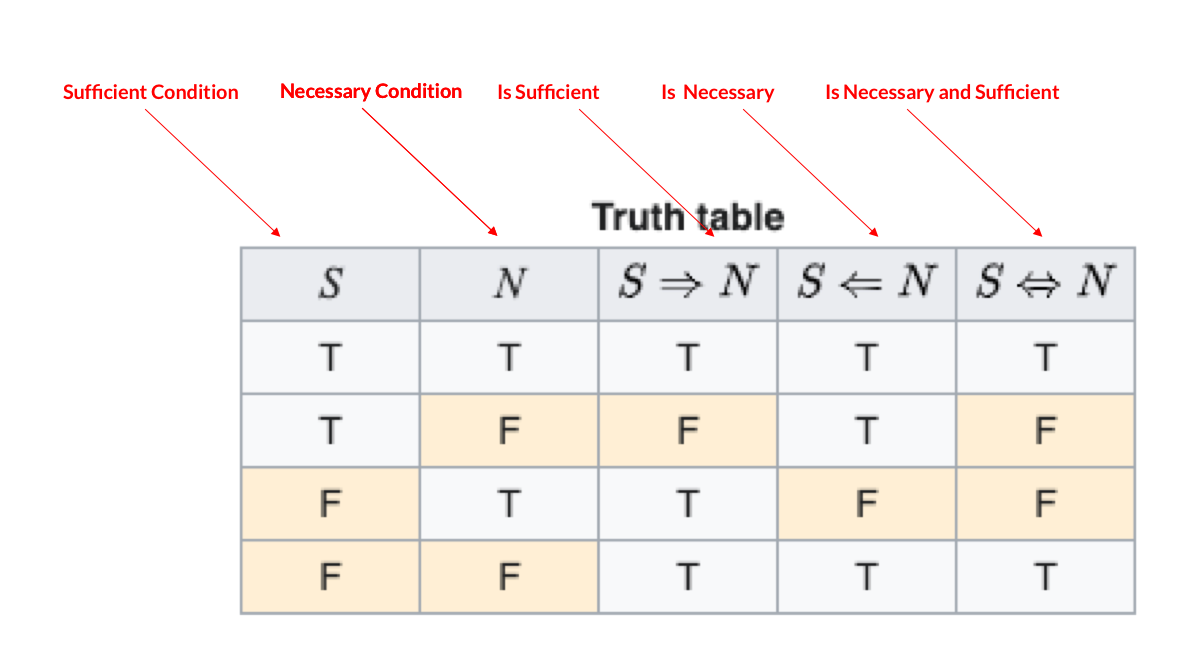
\includegraphics[width=0.8\linewidth]{images/week_10_notes_1_2.png}
                \end{center}
            \end{itemize}
        \end{enumerate}

    \end{mdframed}

    \bigskip

    \underline{\textbf{References}}

    \bigskip

    \begin{enumerate}[1)]
        \item Fayetteville State University: Necessary and Sufficient Conditions, \href{http://faculty.uncfsu.edu/jyoung/necessary_and_sufficient_conditions.htm}{link}
        \item Wikipedia: Necessity and Sufficiency, \href{https://en.wikipedia.org/wiki/Necessity_and_sufficiency}{link}
        \item Wikipedia: Deadlock, \href{https://en.wikipedia.org/wiki/Deadlock#Necessary_conditions}{link}
    \end{enumerate}
    % \item One More Condition
    \item Solutions
    \begin{itemize}
        \item
    \end{itemize}
    % \item Deadlock Prevention
    % \item Preventing Hold and Wait
    % \item Preventing No-Preemption
    % \item Preventing Circular Wait
    % \item Deadlock Avoidance
    % \item Two Avoidance Strategies
    \item Safe States
    \item Unsafe States \& Algorithm
    % \item Restrictions on Avoidance
    % \item Deadlock Detection \& Recovery
    % \item Draw Resource Alloc Graph
    % \item Deadlock Detection
    % \item Deadlock Recovery
    % \item Reality Check
    % \item Why does the Ostrich Algorithm Work?
    \item What is Atomicity?
    \item Why would atomicity fail?
    \item Definitions for Transactions
    \item How to ensure atomicity in the face of failures?
    \item Write-ahead logging
    \item Problems with logging
    % \item Concurrent Transactions
    % \item Conflicting Operations
    % \item Conflict Serializability
    % \item Conflict Serializable?
    % \item Ensuring Serializability
    % \item Example 2 of Phase Locking
    % \item Timestamp Protocols
    % \item Timestamp Ordering
    \item Deadlock and Starvation
    \item Communication Deadlocks
    \item Livelock
\end{itemize}

\end{document}